\chapter{Methods for Network Analysis}

In the current chapter, I will explore the mathematical and statistical techniques that are behind my analysis of the world trade networks. In order to better understand the results that I will show in the next chapter, it is essential to have an understanding not only of the basic concepts of graph theory, but also of the mechanisms and dynamics of the statistical tools that I employ, from the simplest to the more elaborated. I will start by introducing what is a graph (Sec. \ref{sec:4graphtheory}), what are its properties, which metrics we can look at to study it and how we can visualize it to gain knowledge from the plots (Sec \ref{sec:4visualization}). Then I will continue by expanding more on the relevant techinques used for Network Analysis, by presenting the ideas of PageRank, hubs and authorities, and the methods to compute them (Sec. \ref{sec:4pagerank}). Lastly, I will talk about an additional query that one can do on a graph, that is community detection (Sec \ref{sec:4community}): I will explain two methods, Louvain and Stochastic Block Model, that allow one to look for possible communities in graphs, that is to say groups of nodes with similar behavior, like for example a limited group of countries that trades only among them. The following surveys of the statistical techniques I decided to use are adapted from \textcite{barabasi2016network,easley2012networks}.

\section{Intro to Graph Theory}\label{sec:4graphtheory}

If we want to understand a complex system, we first need to know how its components interact with each other or, in other words, we need a map of its wiring diagram.
Let us start by defining formally what is a graph, since it is fundamental for the analysis that will be carried out. 
A \textit{graph} is a way of specifying relationships among a collection of items. It consists of a set of objects, called \textit{nodes}, with certain pairs of these objects connected by links called \textit{edges}. If we denote by $\mathcal{N}$ the set of nodes, and $\mathcal{E}$ the set of edges, then they are sufficient to identify a graph 
\[ 
    \mathcal{G} = (\mathcal{N},\mathcal{E})\,. 
\]
We say that two nodes are \textit{neighbors} if they are connected by an edge. This representation of the network offers a common language to study systems that may differ greatly in nature or scope. The links of a graph can be \textit{directed} or \textit{undirected}: some systems have directed edged, such as the world trade of goods that we analyze in this research where a country imports from another country and the transit of goods has a clear direction, while other systems have undirected edges, like friendship relationships in a social community, where the connection between the entities is mutual (if I am your friend then you are my friend).

A complete description of a graph requires us to keep track of its nodes and edges: this is often done using a so-called \textit{adjacency matrix}. The adjacency matrix $\mathbf{A}$ of a directed graph with $N$ nodes is a $N \times N$ matrix, where $A_{ij} = 1$ if there is an edge going from node $j$ to node $i$, while $A_{ij} = 0$ if there isn't. For an undirected network, the adjacency matrix has the property of being symmetric, i.e. $A_{ij} = A_{ji}$.
\begin{equation}
    A_{ij} = \begin{cases}
        1 & \text{if } (i,j) \in \mathcal{E} \\
        0 & \text{if } (i,j) \notin \mathcal{E}
    \end{cases}
\end{equation}

Another relevant distinction about graphs is whether the edges have a weight assigned to them or not. A network is called \textit{weighted} if each edge $(i,j)$ has a unique weight $w_{ij}$ assigned to it. It is called \textit{unweighted} (or \textit{binary}) if it has no weights assigned, or equivalently if the possible weights are just $\{0,1\}$ (no edge vs. edge). For the \textit{weighted} networks, we can introduce the weighted network matrix $\mathbf{W}$, which has the same size as the adjacency matrix $A$ and whose component are the weights $w_{ij}$.This is the case with the trade networks that we are going to analyze, where the edges between two countries have as weight the monetary value of the exchange, and therefore the element $w_{ij}$ represents the annual amounts of imports per 1000 people from country $i$ to country $j$, measured in euros/1000p.


\subsection{Node properties}
A key property of each node is its \textit{degree}, which is the number of edges that it has that connect to other nodes. We denote by $k_i$ the degree of the $i$-th node in the graph, and we can compute it as 
\[
    k_i = \sum_{j=1}^N a_{ij}
\] 
In our specific case, the degree of a node represents the number of commercial partners that a country has, for either import or export: for example, Italy had a degree of 370 in 2019, meaning that it traded goods with 370 partners in that year.
Since the network under consideration is directed, we make a distinction between \textit{incoming degree} (or \textit{in-degree}) and \textit{outgoing degree} (or \textit{out-degree}):
\begin{itemize}
    \item \textit{in-degree}: denoted by $k_i^{in}$, is the number of edges that point to node $i$, i.e. $\sum_{j=1} a_{ji}$;
    \item \textit{out-degree}: denoted by $k_i^{out}$, is the number of edges that point from node $i$ to other nodes, i.e. $\sum_{j=1} a_{ij}$.
\end{itemize}
The degree $k_i$ of node $i$ can be directly obtained from the elements of the adjacency matrix: if the network is undirected, summing over the rows (or the columns) gives in return a vector of all the node degrees. For a directed network instead, the two sums give different metrics: the sum over the rows gives the incoming degrees, while the sum over the columns the outgoing degrees.

In weighted networks, we can also have a different type of degree centrality, that takes into account the weights of the edges. We call it \textit{weighted degree} (or \textit{strength}) an it corresponds to the sum of the weights of the links of a given node. In our particular case, this alone wouldn't make much sense, since we would be summing together values of imports and exports of a country. So we make a distinction into \textit{weighted in-degree} $k_i^{w,in}$ and \textit{weighted out-degree} $k_i^{w,in}$ as
\begin{align*}
    k_i^{w,in} = \sum_{j=1}^N w_{ji} \\    
    k_i^{w,out} = \sum_{j=1}^N w_{ij} \,.    
\end{align*}
As for the unweighted version, by summing over the rows or the columns of the weighted network matrix $\mathbf{W}$ one can obtain the \textit{weighted in-degree} and \textit{weighted out-degree}, respectively.

Aside from degree centrality measures, one can also investigate for each node how its neighborhood behaves, especially in terms of connectivity among the nodes in it. We can then define another centrality metric called \textit{clustering coefficient}: it represents the extent to which the neighbors of a given node are linked to each other, or in other words, the tendency of a network to form tightly connected neighborhoods. For a node $i$ with degree $k_i$ the local clustering coefficient is
\[
    C_i = \frac{2 L_i}{k_i(k_i-1)}
\]
where $L_i$ is the number of edges among the $k_i$ neighbors of node $i$. The clustering coefficient measures the graph's local edge density: in fact, the more interconnected the neighborhood of node $i$ is, the higher the coefficient. The clustering coefficient is useful in characterizing whether a graph presents features of the \textit{small-world} phenomenon. A network is said to be a \textit{small-world} network if the mean shortest path distance (which is defined right after this) between any pair of nodes is small relative to the total number of nodes in the network (usually, one wants this length to grow no faster than logarithmically as the number of nodes tends to infinity).\\
There are many other centrality measures that are commonly used when studying graphs, especially regarding the notion of path. In a graph, a \textit{path} is a sequence of nodes and edges that start from a given node $i$ and arrive at node $j$. Provided that such path exists, one could also find the \textit{shortest path} between two nodes (the one with fewer edges) among the set of possible paths that connect them. Around the notion of shortest path, we could construct two additional metrics, that are \cite{benedictis2014bacicepii}:
\begin{itemize}
    \item \textbf{Closeness centrality}: it is a measure of how close, in terms of shortest path, a node is with respect to all the other nodes; closeness centrality provides high scores to nodes that are located closer to their set of reachable nodes.
    \item \textbf{Betweenness centrality}: it depicts how well situated a node is in terms of the path that it lies on; that is, a higher score is assigned to nodes that lie on a larger proportion of the whole set of shortest paths among all pairs of nodes. It is a useful measure in the cases when a node is important as an intermediary.
\end{itemize}
Although paths are fundamental concepts in graph theory, in the case of the world trade network under consideration it is hard to attach a meaning to them. The connections among nodes represent imports and exports derived from bilateral relationships, and not long trade routes that go from one country to another, passing through others in the middle. Therefore, for this reason, I've decided not to consider the analysis of these metrics when looking at trade graphs.


\subsection{Graph properties}
Aside from looking at the node degrees one by one, one can also combine them to learn an important property of the graph as a whole, that is the \textit{average degree}. For an undirected network of size N the average degree is 
\[
    k_{avg} = \frac{1}{N}\sum_{i=1}^N k_i = \frac{2 L }{N} 
\]
where $L = 1/2 \sum_{i=1}^N k_i$ is the total number of edges in the graph. The average degree can take values between $0$ and $N-1$, and we have that $k_{avg} = N-1$ only in the case of a fully connected graph, that is a graph where every node is linked to any other node.
If instead we consider a directed graph, we have that the average degree can be computed equivalently either using the in-degrees or the out-degrees
\[
    k_{avg}^{in} = \frac{1}{N} \sum_{i=1}^N k_i^{in} = \frac{1}{N} \sum_{i=1}^N k_i^{out} = k_{avg}^{out}\,,
\]
since the total number of links $L$ is the same if we sum either measures, \textit{in} or \textit{out}. This in fact is true since an outgoing edge from a node is an incoming edge for another.
A second metric that we can compute for the over-all network is the \textit{average clustering coefficient}, which represents the degree of clustering of the whole network:
\[
    C_{avg} = \frac{1}{N} \sum_{i=1}^N C_i \,;
\]
This aggregated metric gives us an idea of the level of interconnectedness of the graph as a whole, which emerges from the connectedness of the local clusters. 
A closely related measure to the average clustering coefficient that can be computed on a graph to have an idea of how well it's connected is the \textit{density}: it is defined as the proportion of edges that are present in the graph over the total possible number of edges that could be formed. 
For a directed graph, it is defined formally as
\[
    D = \frac{L}{2\binom{N}{2}} = \frac{L}{N(N-1)}
\]
where $L$ is the total number of edges in the graph, and $N$ is the total number of nodes. The density of a graph goes from 0, if there are no edges at all, to 1, if all possible edges are present, in which case we say that the graph is \textit{complete}. In real networks, the number of nodes $N$ and the number of edges $L$ can vary widely, but more often than not the network that we observe are \textit{sparse}, meaning that their density is low \cite{barabasi2016network}. This also means that the adjacency matrix is sparse, containing a lot of zeros. In fact, this is the case with the world trade network that we take under study: even the most central and connected nodes are not linked with the majority of the other countries.


\subsection{Degree distribution and power law}
Given all the degrees of the nodes in the graph, we can also introduce the \textit{degree distribution} $p_k$ of the nodes, which is a discrete distribution indicating the probability that a randomly selected node has degree $k$. For a network of $N$ nodes, the degree distribution is the normalized histogram given by 
\[ 
    p_k = \frac{N_k}{N} 
\]
where $N_k$ is the number of nodes that have degree $k$. 
The degree distribution is a characteristic of the network structure and can have different functional forms. For example, random networks have a binomial degree distribution, while regular networks, where all the nodes have the same degree, have a distribution concentrated at a single value (delta function at that degree) \cite{sajedianfard2021quantitative}. Observing the structure of the degree distribution can yield a lot of relevant information about a network, such as whether it displays behaviors of the \textit{small-world} phenomenon or the \textit{scale-free} property.
While performing the analysis, it will be of interest to study each graph's degree distribution, to observe whether they express known behaviors. In particular, as \textcite{barabasi2016network} points out, many real networks like the world trade web that we are studying, are prone to have a power-law degree distribution, which is
\[
    p_k \sim k^{-\gamma} \text{ or equivalently } \log(p_k) \sim -\gamma \log(k) \,.
\]
The exponent $\gamma$ is called \textit{degree exponent}, and it indicates how much rapidly the probability decreases as $k$ increases. A power-law distribution over the degrees is characterized by a very high frequency of nodes with low degree and a low presence of nodes with considerably high degree. This is called the \textit{scale-free} property and one can verify that a network shows it by means of a log-log plot of the degree frequencies: if they can be approximated by a straight line (as in the above formulation), then we can say that they follow a power-law distribution.
Another perspective that we can consider is to look at the weighted degrees, to assume that they were generated by a distribution, and then study its properties. To do so, one can approximate the distribution via a histogram on the vector of weighted degrees (in or out) and then use the obtained histogram as an estimate of the ``real" distribution, thus computing qualitative and quantitative properties. Similarly to the unweighted version, we could again study whether the behavior of the histogram resembles a power law, where in our specific case it would mean that there are a lot of trade exchanges with low value, while a small number of the imports instead have very high amounts of traded goods. In the following chapter, we will perform both of these analyses, trying to fit a power law on the unweighted and weighted degree distributions.


%\pagebreak
\section{Trade Networks Visualization}\label{sec:4visualization}

As it was previously shown in Section \ref{sec:ch3graphs} through the graph plots, a lot of insights and information can be gained through the visualization of the network. If we restrict our attention to the datasets and the tables, we can have an idea of the countries that play a major role in the global trade, and we receive the impression of the significance of the economic exchanges. However, we struggle to have a comprehensive view of the effects of these interactions on each other: for this reason, we make use of a graph which is able to capture and represent this type of intricate relationships. In order to convey meaningful information, we need to spend special attention to how we display a graph. Since we are dealing with countries and imports, the most natural way to represent a world graph would be to use the geographical information of each nation: we collocate each node on the coordinates of the centroid of that country, and then we add the links among the countries (as in Figure \ref{fig:geograph}).
\begin{figure}
    \centering
    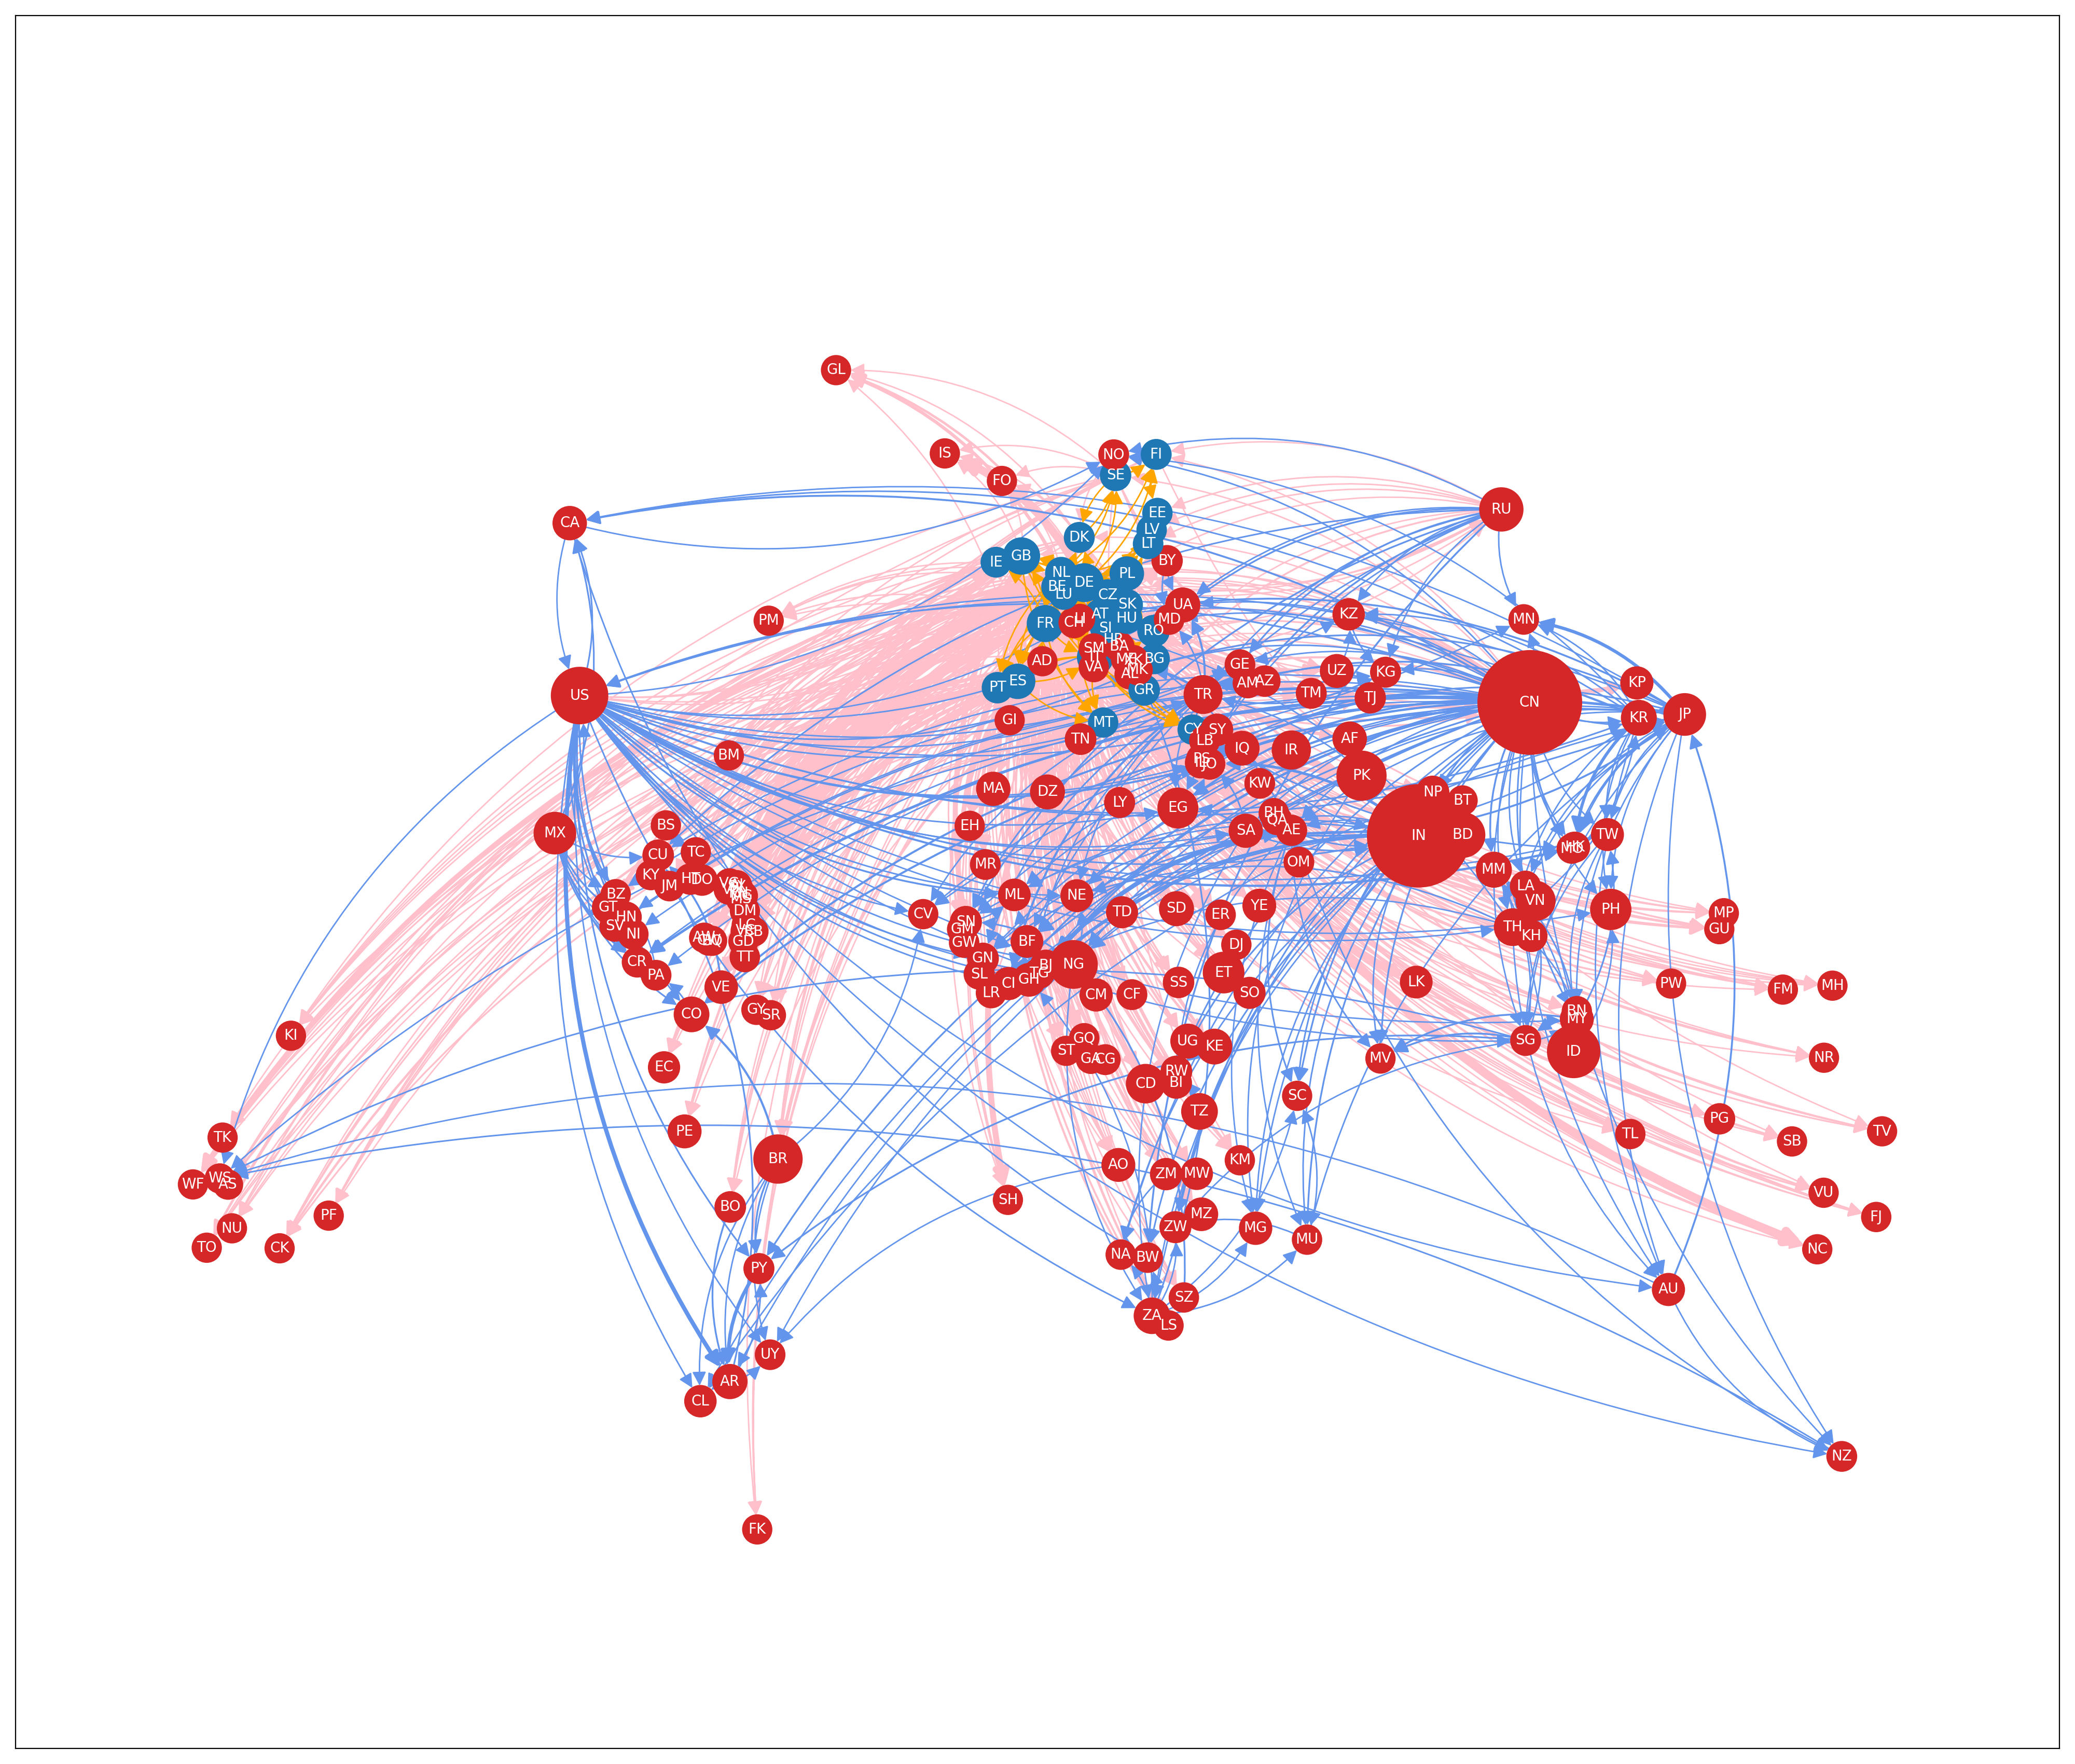
\includegraphics[width=\textwidth]{pics/full_y19_pTO_geo.png}
    \caption[Global trade network of all products in 2019.]{Global trade network of all products in 2019. Nodes are positioned according to the geographical location of the country, and their size is proportional to the population. The color of the node indicates EU countries (\textit{blue}) and non-EU (\textit{red}); the color of the edge is \textit{orange} for intra-EU exchanges, \textit{pink} for EU - non-EU exchanges and \textit{azure} for extra-EU exchanges. Only the top 5 import partnership for each country are shown.}
    \label{fig:geograph}
\end{figure}
What we can see in this plot is the complex net of trade routes among countries all around the world, and it emerges the important role that the greatest economies such as the US and China play in the global scenario. On the contrary, since all the blue nodes belonging to the European Union are so close to each other, it is impossible to see the web of intra-EU exchanges. What \textcite{benedictis2014bacicepii} point out, in fact, is that this picture does not give full account of the implication of the interdependence among countries, and using geographical positions we can draw conclusions only about the bilateral trades of countries, not their ensemble. In their words, ``\textit{this is the visual analog of the assumption of conditional independence among dyads imposed on international trade flows}".
If we want countries' interactions to be accounted in determining the relative position of each nation in the whole trading network, we should ignore their geographical position and move from a physical space to a \textit{topological space}. In the following part, we will employ Network Analysis methods to carry out this goal and improve the visualization of the graph.

\subsection{Force-Directed Algorithms}
Instead of using the geographical position of the countries, we can apply what is called a \textit{force-directed} algorithm to plot the nodes of the graph. In brief, this kind of algorithms act as a balanced spring system that minimizes the energy in the system: it is as if countries were linked through springs. Countries which are connected with an edge tend to stay close (as if there were a force that attracts them), while countries which are not connected tend to be placed far apart. In doing so, the position of each country does not depend only on its links but also on the indirect effect of its neighbors' neighbors: this is to say that countries are not affected just by their trade partners but also by entire groups or clusters of countries. In particular, the technique that we apply here is the one proposed by \textcite{fruchterman1991graph}.
The main consequence of this method is that we can now interpret the position of nodes relatively to all the other countries in the trade graph. This is an added benefit, since we can observe the effect of a relationship between any two trading countries and the whole structure of the network itself, showing patterns that were difficult to see in the previous visualization. An example of this can be seen in Figure \ref{fig:forcedir}, which displays the same graph as before, but with a spring layout from the force-directed algorithm.
\begin{figure}
    \centering
    \includegraphics[width=\textwidth]{pics/full_y19_pTO_force_20.png}
    \caption[Global trade network of all products in 2019.]{Global trade network of all products in 2019. Nodes are positioned according to the force-directed algorithm, and their size is proportional to the population. The color of the node indicates EU countries (\textit{blue}) and non-EU (\textit{red}); the color of the edge is \textit{orange} for intra-EU exchanges, \textit{pink} for EU - non-EU exchanges and \textit{azure} for extra-EU exchanges. Only the top 5 import partnership for each country are shown.}
    \label{fig:forcedir}
\end{figure}
By construction, each node has only 5 incoming links, which is equivalent to say that their in-degree is 5. The weights of these edges change depending on the strength of the partnership, which in our case is measured in average expense for 1000 inhabitants. If on the one hand the in-degree is fixed, we cannot say the same in advance for the out-degree, and it is this difference across countries which plays a key role in the visualization layout. Highly connected nodes are generally placed at the center of the network, while countries which are less connected are placed near the borders of the figure. For a node to have many links means that a lot of countries have it in their top-5 list of importing partners. In the figure, we can spot these nodes easily, since they are the most central ones, such as China (CN), the United States (US) and Germany (DE). We see that a lot of links origin from these nodes and go towards both near and peripheral countries, and in fact, being tied to many nodes is the reason why the layout has put them in a central position. A network with this structure is called \textit{core-periphery}. In general, this structure consists of a core cluster which is internally cohesive, and one or more other positions with ties to the core cluster, but not to each other. These peripheral positions may or may not be internally cohesive \cite{wasserman1994social}. This resembles the network in Figure \ref{fig:forcedir}, where all the countries which are at the periphery of the graph are linked with the more important economies at the center, while this center countries have a high level of connections among them.
A second thing that we can observe by comparing the two plots is the impact of \textit{pink} edges, i.e. exchanges between one EU and one non-EU country. While in the first plot we see that the European Union has a great number of exchanges with south-American countries and Pacific islands, this web does not appear more important than the \textit{azure} links (among extra-EU). When we move instead to the second visualization, the comparison is much more evident: the ratio of pink edges against azure ones breaks in favor of the former and it is easier to see that a high number of peripheral nations trade considerably with the EU. In fact, the number of pink edges in this specific case is 699, while the number of azure ones is 320. 
A final relevant information is conveyed by the size of the nodes: since we use population as the normalizing constant for the weight of the edges, in both plots a bigger node represents a more populous country. Showing it in the visualization allows us to compare more easily countries with similar size. For example, we can compare China (CN) and India (IN), the two biggest nations in terms of inhabitants, and we immediately see that in terms of exports China has a more central role in the world network than India: in fact, the out-degree of China is 78 while that of India is 22.\\
Given all the reasons that are explained in this paragraph, it is easy to see that the kind of layouts using force-directed algorithms are much more informative than the ones on the geographical space. Hence, from here onward, all graphs will be plotted in this way.


%\pagebreak
\section{PageRank, Hubs and Authorities}\label{sec:4pagerank}

In the world trade network, most countries are characterized by weak trade links, but there exists a group of advanced countries featuring a large number of strong relationships \cite{deguchi2014hubs}, which suggests a core-periphery structure \cite{fagiolo2010evolution}. As pointed out before, we can have an understanding of the network by looking at the centrality measures of its nodes (in- and out-degree) or of the entire graph (average degree, density). However, node degrees are computed using only local information, since for every node it is enough to know the connections with its neighbors. Let me introduce now a centrality measure that instead takes into account the relationships of the entire network and their effect on the node under consideration: the PageRank. 
First introduced by \textcite{page1999pagerank}, this measure of centrality of a node is influenced by the same measure for the neighboring nodes, and it is proportional to their PageRank divided by their out-degree. What this means is that nodes which point to many others give only a small amount of centrality on to each of those others, even if their own centrality is high. Hence, to compute a node's PageRank we need to know its neighbors' PageRank, and so on, showing the fact that the information for each single node comes from the whole graph. Intuitively, we can think of PageRank as a kind of ``fluid" that circulates through the network, passing from node to node across edges following their direction, and accumulating at the nodes which are most important \cite{easley2012networks}. To be more precise, we compute PageRank ($pr$) in the following way:
\begin{enumerate}
    \item Given a graph with $n$ nodes, we start by assigning to all nodes the same initial value for $pr$, set to $1/n$;
    \item Choose a number $k$ of iterations, and for $k$ steps repeat:\\
            Each node divides its current $pr$ equally across its out-going links, and passes these equal shares to the pages it points to. Each node updates its new $pr$ as the sum of the shares that it receives from the neighbors.
\end{enumerate}
One can prove that (except in certain degenerate cases) the PageRank values of all nodes converge to limiting values as the number of steps $k$ goes to infinity. To avoid cases in which the total available $pr$ in the network ends up in nodes that have no link that can give it back, we can introduce a \textit{scaled} version of the PageRank, whose formula is
\begin{equation}\label{eq:pagerank}
    pr_i = \alpha \sum_{j} a_{ij} \frac{pr_j}{k_j^{out}} + \beta
\end{equation}
where $\alpha$ and $\beta$ are positive constants, $a_{ij}$ is an entry of the adjacency matrix and $pr_i$ and $pr_j$ are the PageRank values of nodes $i$ and $j$, respectively. 
The economic significance of this centrality measure is that a country with high PageRank centrality is connected to a central country, which is also a country with high PageRank centrality, indicating that they are core sources in that specific market.
An alternative way to define the PageRank of a graph is the eigenvector of the following Google matrix:
\begin{equation}\label{eq:googlemat}
    g_{ij} = q \frac{a_{ij}}{\sum a_{ij}} + (1-q)\frac{1}{N}
\end{equation}
Here $q = 0.85$ is a positive parameter introduced to ensure the existence of a unique solution. If we denote by $\mathbf{G}$ the Google matrix defined above, then we can obtain the vector of PageRank values $\mathbf{z} = (z_1,\dots,z_N)^T$ by repeating the following iteration until convergence:
\begin{equation}
    \mathbf{z(t+1) = G^T z(t)}
\end{equation}
In recent years, a major topic in network science research has been the investigation of the effects of ranking algorithms on the performance and behavior of networked systems. \textcite{ermann2011google} found that the page rank approach gives a ranking that is independent of the trade amount of a given country.
PageRank centrality assigns high centrality values to those nodes which have a high number of incoming edges from other nodes with high centrality. In terms of countries and trade, a country has high PageRank if it imports from other countries with high PageRank. Countries instead which have a high number of outgoing links with a large amount of trade, and hence have low values of PageRank, are called \textit{hubs}. In the next paragraph I will show how to find countries which are hubs and their interpretation.

\paragraph{Hubs and Authorities}
According to what is reported by \textcite{deguchi2014hubs}, an economic \textit{hub} country usually imports raw materials, parts, and intermediate goods from other countries, assembles final goods and exports these goods to other countries. % Maybe talk about China being a hub country, if verified
Therefore, differently from the PageRank importance, we can also define a node's centrality based on whether it \textit{points to} other countries with high importance, which in our case is a country that exports to other central countries \cite{sajedianfard2021quantitative}. On the other hand, we could define the importance of a node based on whether it is \textit{pointed at} by many others. Following this line, we could differentiate the types of central countries that we can find in networks, and we call them:
\begin{itemize}
    \item \textbf{\textit{Hubs}}: The countries that trade with important and central points (with respect to that specific trade market) and they export to other important and central countries (the authorities) of the network;
    \item \textbf{\textit{Authorities}} The countries that are important and central points of a specific trade market in the import sector.
\end{itemize}
To put it simply, a node with a high authority value is pointed to by many other nodes with high hub values, and a node with a high hub value points to many nodes with high authority values. Note however that an authority may also be a hub and vice versa. In the context of the world trade network, authorities are countries that receive a lot of imports, from many countries, and thus are dependent from them for that specific product. Contrary to what the name suggests, very often countries with high authority values are small countries that completely depend on imports from others for their demand of goods. Instead, hubs are countries that are typically producers or manufacturers of goods and that export those goods to a high number of other countries.
To compute the hub and authority values of the nodes in the network, I use an algorithm called Hyperlink-Induced Topic Search (HITS), which was originally introduced by \textcite{kleinberg1999authoritative}. Let me define the vector of HITS authority values as $\mathbf{x}=(x_1,\cdots,x_N)^T$, and the vector of HITS hubs as $\mathbf{y}=(y_1,\cdots,y_N)^T$. Similarly to the $pr$ values, the two metrics are defined by the limit of the following set of iterations:
\begin{align}\label{eq:hits}
    \mathbf{x}^{t+1} &= c(t) \mathbf{A}^T \mathbf{y}^t \\
    \mathbf{y}^{t+1} &= d(t) \mathbf{A} \mathbf{x}^{t+1} 
\end{align}
where $c(t)$ and $d(t)$ are normalization factors to force the sums of all elements equal to one, as we impose that for every $t$
\begin{align*}
    \sum_{i=1}^N x_i^{t} = 1 \\
    \sum_{i=1}^N y_i^{t} = 1 \,.
\end{align*}
The initial values of the iterations are $x_i = 1/N$ and $y_i = 1/N$ for all nodes $i$. What can be seen from Equation \ref{eq:hits} is that the HITS authority vector $\mathbf{x}$ is the eigenvector of the matrix $\mathbf{A^T A}$, while the HITS hub vector $\mathbf{y}$ is the eigenvector of $\mathbf{A A^T}$ \cite{deguchi2014hubs}.

\section{Community detection}\label{sec:4community}
A fundamental modern technique in the analysis of network data is the automatic discovery of communities, which are groups of nodes that are strongly connected or that share similar features or roles. However, community detection is a rich and challenging problem since there is no clear definition on what constitutes a community: usually, communities are defined as non-overlapping groups of nodes such that there are more edges within groups than between them, but this definition doesn't cover all cases and leaves space to many computationally approaches to detect them \cite{fortunato202220years}. In the next sections, I will overview two of the most common approaches: the \textit{Louvain method} and the \textit{Stochastic Block Model}. 
The first approach is based on an optimization problem: we have a function that, given a division of the network in communities, returns a score such that a ``good" division gets a higher score, and our goal is to maximize it. The most common score is the quality function known as modularity, which explicitly favors divisions with many edges within groups.
The second approach instead is based on statistical inference, where we assume that communities are not just a feature of the network structure, but a primary driver of it. Nodes are connected precisely because of the community they belong to, and not the other way around. The placement of edges is represented using a probabilistic model, in which the probability that two nodes are connected depends uniquely on the communities they belong to. A ``good" community structure is one who has a high probability of generating the observed network through the model, so that we can use this probability as a score function.
These are the two approaches for community detection that I will apply to the world trade networks, in order to see whether I can uncover any underlying structure of the trade relationships that is not apparent from a qualitative view of the graph or through the other metrics that I have described so far in the chapter.

\subsection{Louvain method}

The Louvain Community Detection algorithm, or Louvain method, is a simple optimization method to extract the community structure of a network. It is a heuristic method whose goal is to maximize the \textit{modularity} function. The modularity of a network is a measure of the structure of the graph, which quantifies the strength of the division of the nodes into modules (i.e. communities). In general, networks with high modularity have dense connections between the nodes within a community but sparse connections between nodes in different communities.
For weighted directed networks, the formulation of modularity is 
\[
    Q = \frac{1}{m} \sum_{ij} \left[ W_{ij} - \frac{k_i^{in}k_j^{out}}{m} \right] \delta(c_i,c_j)
\]
where $W_{ij}$ is the weight of the edge $(i,j)$, $k^{in}$ and $k^{out}$
are the in-degree and out-degree of nodes, $c_i$ indicates the community of node i and the $\delta$-function $\delta(c_i,c_j)$ is equal to 1 if $c_i=c_j$ or $0$ otherwise \cite{leicht2008community}.
Therefore, we use Louvain algorithm to find the configuration of communities that maximizes modularity. Starting from a weighted directed network of $N$ nodes, the method works in two phases. 
In the first phase, we start by assigning a different community to each node of the graph, thus starting with as many communities as nodes. Then for each node $i$ we consider the neighbors $j$ of $i$ and we evaluate the gain in modularity that would take place by removing $i$ from its community and adding it to the community of $j$. Then, node $i$ is placed in the community such that we have the greatest positive gain possible in modularity, otherwise $i$ stays in the original community if there is no improvement \cite{blondel2008louvain}. We can directly compute the modularity gain $\Delta Q$ obtained by moving an isolated node \(i\) into a community \(C\) as
\[
    \Delta Q = \frac{k_{i,in}}{m} - \gamma\frac{k_i^{out} \cdot\Sigma_{tot}^{in} + k_i^{in} \cdot \Sigma_{tot}^{out}}{m^2}
\]
where \(k_i^{out}\), \(k_i^{in}\) are the outer and inner weighted degrees of node \(i\) and \(\Sigma_{tot}^{in}\), \(\Sigma_{tot}^{out}\) are the sum of in-going and out-going links incident to nodes in \(C\).
The parameter $\gamma$ is called \textit{resolution}, and its function is to assign a preference to larger (when $\gamma < 1$) or smaller (when $\gamma > 1$) communities \cite{hagberg2008networkx}.
This process is repeated sequentially for all nodes until we have no more improvement available and the first phase is complete.
The second phase then consists in creating an auxiliary network whose nodes are now the communities found during the first phase. The weights of the edges between the new nodes are given the sum of the weight of the edges between nodes in the corresponding two communities (links between nodes of the same community lead to self-loops in the new network). Once the network is constructed, we can reapply the first phase and construct new communities. Denoting by \textit{pass} each two-phase step of the optimization, we note that by construction the number of communities decreases at each pass. We iterate each pass until there are no more changes that induce a gain in modularity, and this means we have reached a maximum \cite{blondel2008louvain}.


%\pagebreak
\subsection{Stochastic Block Model}\label{sec:sbm}
Stochastic block models (SBM) are an increasingly popular class of models in the field of statistical analysis of graphs and networks. They can be used to discover or understand the latent structure of a network, as well as for clustering purposes. In our particular case, I will apply this method on the trade graphs to discover if any communities or clusters emerge and find an interpretation for them.
I will proceed now to describe a formal version of the stochastic block model, together with the needed terminology. This part is adapted from \textcite{lee2019review}.\\
Let us consider a graph $\mathcal{G} = (\mathcal{N},\mathcal{E})$, where $\mathcal{N}$ is the node set of size $N = |\mathcal{N}|$, and $\mathcal{E}$ is the edge set of size $M = |\mathcal{E}|$. Taking two nodes $p$ and $q$ from $\mathcal{N}$, we call a pair of nodes a \textit{dyad}, and the existence of an edge for the dyad $(p,q)$ is denoted by $\mathbf{A}_{pq}$ which is an element of the $N \times N$ adjacency matrix $\mathbf{A}$. Recall that if $\mathcal{G}$ is directed, as in our case, then the adjacency matrix is not symmetric and $\mathbf{A}_{pq}$ is independent of $\mathbf{A}_{qp}$.
In the SBM, each node belongs to one of the $K$ groups (which are less than $N$): since the groups are unknown before modeling, for nodes $p = 1,\ldots,N$ we also define a vector $\mathbf{Z}_p$ of dimension $K$ which is a one-hot vector representing the membership of node $p$. This means that all the elements of $\mathbf{Z}_{p}$ are $0$ except for one position, call it $k$, which is equal to $1$, signifying that node $p$ belongs to group $k$.
Similar to $\mathbf{Z}_{p}$, we also define a $N \times K$ matrix $\mathbf{Z}$ as
\[
    \mathbf{Z} = (\mathbf{Z}_1 \cdots \mathbf{Z}_n)^T
\]
where we call $\mathbf{Z}_{pi}$ the $i$-th element of $\mathbf{Z}_p$.\\
If we take $\mathbf{Z}$ and we sum over the rows, then we can obtain a vector $\mathbf{N} = (N_1 \cdots N_K)^T$ of the group sizes, since the vectors $\mathbf{Z}_{p}$ are zero-one.
In order to describe the generation of the edges of $\mathcal{G}$ according to the group the nodes belong to, we introduce a $K \times K$ block matrix $\mathbf{C}$. Given that $\mathcal{G}$ is directed, we have that for every community $1 \leq i,j \leq K$, $\mathbf{C}_{ij}$ represents the probability of having a directed edge from a node in $i$ to a node in $j$. The idea of the block matrix $\mathbf{C}$ is that the dyads are conditionally independent given the group memberships $\mathbf{Z}$. Equivalently, we could also say that
\[
    \mathbf{A}_{pq} \sim Bernoulli(\mathbf{Z}^T_p \mathbf{C} \mathbf{Z}_q),
\]
that is to say that $\mathbf{A}_{pq}$ follows a Bernoulli distribution where the success probability is the probability of having a node between the two groups to which $p$ and $q$ belong to. Furthermore, $\mathbf{A}_{pq}$ is independent of $\mathbf{A}_{rs}$ for $(p,q) \neq (r,s)$, given $\mathbf{Z}_p$ and $\mathbf{Z}_q$.\\
The assumption that the edge probability of a dyad depends only on their memberships is based on the concept of \textit{stochastic equivalence}: for nodes $p$ and $q$ in the same group, the probability of $p$ connecting with node $r$ is equal and independent to the probability of $q$ connected with $r$. This concept does not require that the nodes in the same group are more connected within themselves than with nodes in another group, but essentially it means that they express the same characteristics in terms of which nodes (of which group) they are connected to. We can also say this by noting that the elements among the major diagonal of $\mathbf{C}$ are not necessarily higher than the off-diagonal elements.\\
Given $\mathbf{Z}$ and $\mathbf{C}$, and given the assumption that the edges are Bernoulli distributed conditional on the group memberships, then we can write down the likelihood as 
\begin{equation}\label{eq:sbmlik}
    \pi (\mathbf{A}|\mathbf{Z},\mathbf{C}) = \prod_{p\neq q}^n \pi(\mathbf{A}_{pq}|\mathbf{Z},\mathbf{c}) 
    = \prod_{p\neq q}^n \left[ \left( \mathbf{Z}^T_p \mathbf{C} \mathbf{Z}_q \right)^{\mathbf{A}_{pq}} \left( 1 - \mathbf{Z}^T_p \mathbf{C} \mathbf{Z}_q \right)^{(1-\mathbf{A}_{pq})} \right]
\end{equation}
By applying a change of index, we can rewrite \ref{eq:sbmlik} as
\begin{equation}
    \pi (\mathbf{A}|\mathbf{Z},\mathbf{C}) = \prod_{i \leq j} \mathbf{C}^{\mathbf{E}_{ij}}_{ij} (1 - \mathbf{C}_{ij})^{(\mathbf{N}_{ij} - \mathbf{E}_{ij})}
\end{equation}
where we have that $\mathbf{E}$ is a $K \times K$ adjacency matrix between groups, i.e. $E_{ij}$ is the number of edges going from block $i$ to block $j$ in the case of directed graphs. We also have $\mathbf{N}_{ij} = \mathbf{N}_i\mathbf{N}_j$ if $i \neq j$, $\mathbf{N}_{ij} = \mathbf{N}_i(\mathbf{N}_i-1)$ if $i=j$.\\
When applying SBMs to real-world data, such as in our case, usually neither $\mathbf{Z}$ nor $\mathbf{C}$ is known, and they have to be inferred, therefore we need to make assumption before modelling. For $p = 1,...,n$, we assume that the latent variable $\mathbf{Z}_p$ is independent of $\mathbf{Z}_q$ a priori. We also assume that $P(\mathbf{Z}_{pi}=1) = \theta_i$, where $\theta_i$ is the $i$-th element of the $K$-vector $\mathbf{\theta} = (\theta_1 \dots \theta_K)^T$ such that $\sum_{i=1}^K \theta_i = 1$. Essentially, we could say that the latent group $\mathbf{Z}_p$ follows the multinomial distribution with probabilities $\mathbf{\theta}$, that is
\begin{equation}
    \pi(\mathbf{Z}|\theta) = \prod_{p=1}^n \mathbf{Z}_p^T \theta = \prod_{p=1}^n \theta^T \mathbf{Z}_p = \prod_{i=1}^K \theta^{N_i}_i
\end{equation}

\subsubsection{Degree-Corrected SBM}
A variant of the previously shown SBM is the Degree Corrected SBM, proposed by \textcite{karrer2011dcsbm}. Here the authors are working with multigraphs, and they propose to redefine $\mathbf{A}_{pq}$ to be the number of edges for the dyad $(p,q)$ and they assume it follows a Poisson distribution, while $\mathbf{C}_{ij}$ is the \textit{expected} number of edges from a node in group $i$ to a node in group $j$. The density of $\mathbf{A}_{pq}$ becomes
\begin{equation}\label{eq:poisSBMdens}
    \pi(\mathbf{A}_{pq}|\mathbf{Z,C}) = (\mathbf{A}_{pq}!)^{-1} \exp \left( -\mathbf{Z}^T_p \mathbf{C} \mathbf{Z}_q \right) \left( \mathbf{Z}^T_p \mathbf{C} \mathbf{Z}_q \right)^{\mathbf{A}_{pq}}
\end{equation}
What they claim is that in the limit of a large sparse graph, the edge probability equals the expected number of edges, therefore this version of the SBM (called Poisson SBM) is asymptotically equivalent to the Bernoulli counterpart, presented above.\\
Their proposal, however, doesn't stop here, since so far we have just changed the likelihood of the model. What they introduce is a new parameter $\phi_p$ for each node $p$: the $\phi$'s are subject to the constraint that $\sum_{p=1}^N \phi_p \mathbb{1}\{\mathbf{Z}_{pi} = 1\} = 1$ for every group $i$, so that the expected number of edges for the dyad $(p,q)$ is now $\phi_p \phi_q \mathbf{Z}^T_p \mathbf{C} \mathbf{Z}_q$. Thus, the density of $Y_{pq}$ in \ref{eq:poisSBMdens} becomes
\begin{equation}\label{eq:dcsbm}
    \pi(\mathbf{A}_{pq}|\mathbf{Z,C,\phi}) = (\mathbf{A}_{pq}!)^{-1} \exp \left( -\phi_p \phi_q \mathbf{Z}^T_p \mathbf{C} \mathbf{Z}_q \right) \left(\phi_p \phi_q \mathbf{Z}^T_p \mathbf{C} \mathbf{Z}_q \right)^{\mathbf{A}_{pq}}
\end{equation}
where $\mathbf{\phi} = (\phi_1 \cdots \phi_N)^T$.\\
Equation \ref{eq:dcsbm} is what is called the Degree-Corrected (DC) SBM. We can interpret the parameters $\phi_p$ and $\mathbf{C}_{ij}$ as their maximum likelihood estimates: $\phi_p$ can be seen as the ratio of the degree of $p$ to the sum of the degrees in $p$'s block, while $\mathbf{C}_{ij}$ as the total number of edges between groups $i$ and $j$ \cite{lee2019review}.
% As in the Bernoulli version, also here we can rewrite the likelihood based on the equation above by making a change of indices from nodes $p,q$ to blocks $i,j$ as
% \begin{equation}
%     \pi(\mathbf{A}|\mathbf{Z,C,\phi}) = \prod_{p<q}^N (\mathbf{A}_{pq}!)^{-1} \exp \left( -\phi_p \phi_q \mathbf{Z}^T_p \mathbf{C} \mathbf{Z}_q \right) \left(\phi_p \phi_q \mathbf{Z}^T_p \mathbf{C} \mathbf{Z}_q \right)^{\mathbf{A}_{pq}}
% \end{equation}
What \textcite{karrer2011dcsbm} argue in their paper for DCSBM is that the simple block model doesn't work well in many applications to real world networks, and in particular, it is not flexible enough to generate graphs with structure similar to that found in empirical data. This means that community detection, seen here as \textit{a posteriori} fit of the model to the data, gives poor results, since in fact in the original SBM the expected degree is the same for all nodes in each group. The simple variation that they introduce is to include heterogeneity in the degrees of vertices, and they show that in this way they are able to improve the performance of the models for statistical inference of group structure.

